\section{Home-Page - Rollen:Alle}
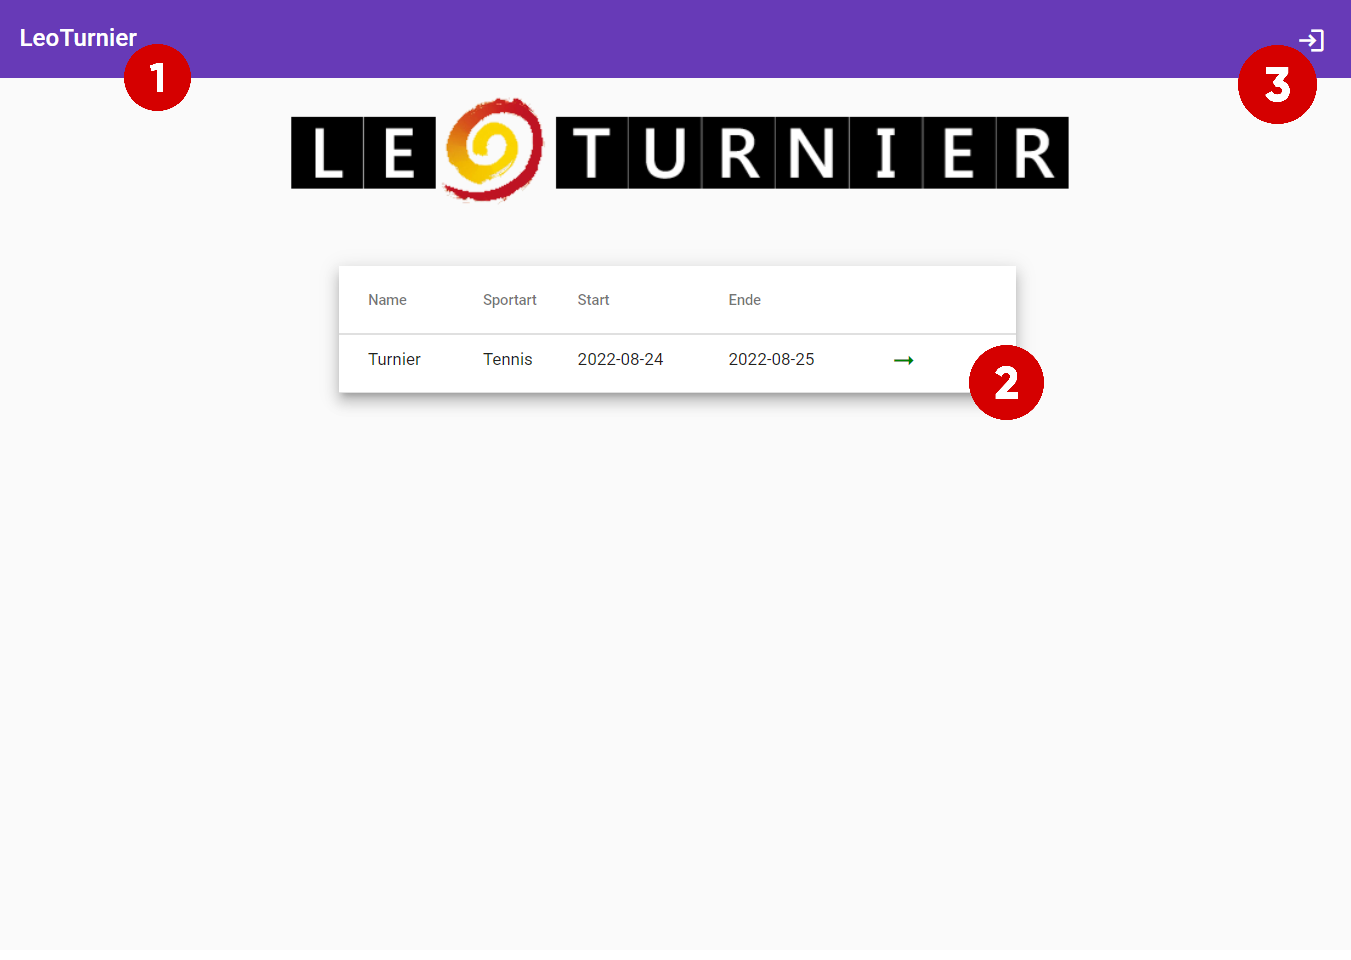
\includegraphics[scale=0.4]{pics/user-guide/homepage.png}
\bigskip


\includegraphics[scale=0.05]{pics/user-guide/numbers/number-1.png} \begin{LARGE} Titel \end{LARGE}

Links oben wird dauerhaft der Titel LeoTurnier gezeigt dieser dient auch gleichzeitig als Homebutton,
also kommt man per Knopfdruck immer wieder auf diese Seite.
\bigskip


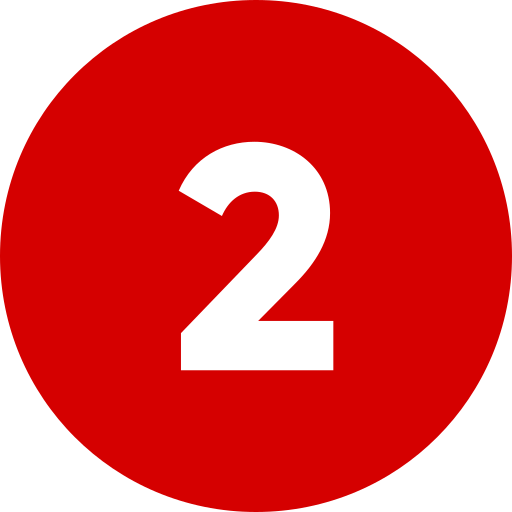
\includegraphics[scale=0.05]{pics/user-guide/numbers/number-2.png} \begin{LARGE} Laufenden Turniere \end{LARGE}

In dieser Tabelle werden alle laufenden Turniere angezeigt. Zu jedem Turnier werden die Sportart, das Startdatum und das Enddatum angezeigt,
sollten diese eingetragen sein. (\textit{Nur der Name und der Modus sind zur Erstellung nötig})

Mit dem rechten grünen Pfeil kommen Sie zur Tournament-View-Page(5.2) des jeweiligen Turniers.
\bigskip

\newpage

\includegraphics[scale=0.05]{pics/user-guide/numbers/number-3.png} \begin{LARGE} Login Button \end{LARGE}

Um Turniere zu erstellen und verwalten zu können ist es nötig sich vorher einzuloggen. Mit diesem Button sollten Sie direkt zum Keycloak weitergeleitet werden um sich mit ihrem Username und Password zu authorisieren.
Danach werden Sie zur Login-Page(5.3) weitergeleitet werden.

\newpage
\section{Tournament-View-Page - Rollen: Alle}

Es gibt 2 Arten von Tournament-View-Pages:
\begin{itemize}
    \item Table-View (für den Round Robin Modus)
    \item Tree-View (für den Elimination Modus)
\end{itemize}

\subsection{Tree-View}
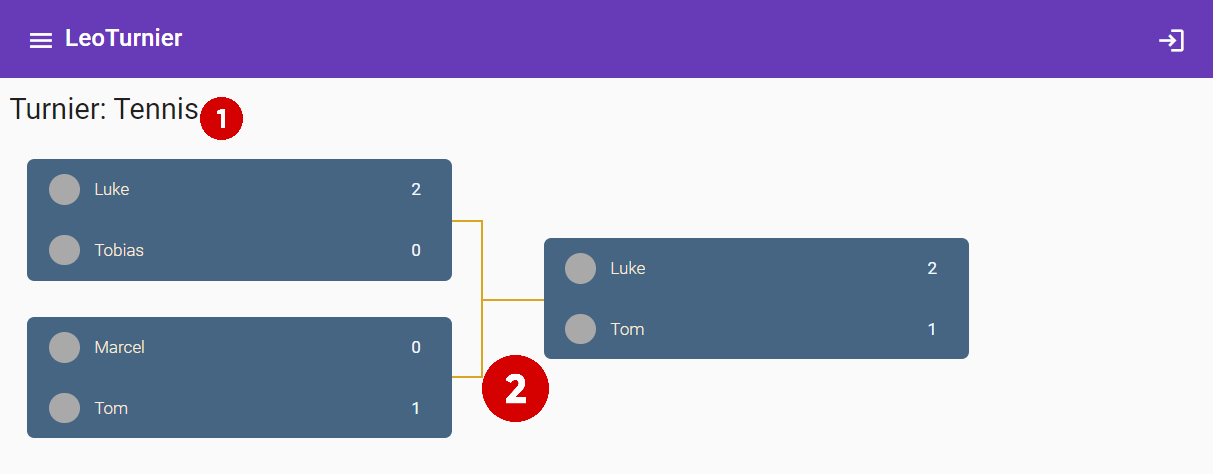
\includegraphics[scale=0.4]{pics/user-guide/tree-view.png}
\bigskip


\includegraphics[scale=0.05]{pics/user-guide/numbers/number-1.png} \begin{LARGE} Info \end{LARGE}

Hier finden Sie eine kurze Info zum Turniernamen und Sportart
\bigskip

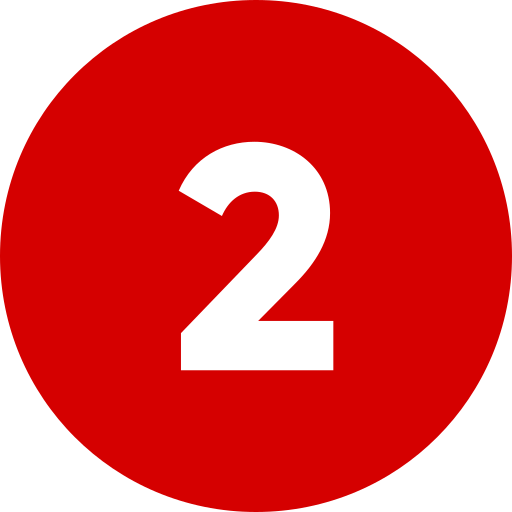
\includegraphics[scale=0.05]{pics/user-guide/numbers/number-2.png} \begin{LARGE} Turnierbaum \end{LARGE}

Hier finden Sie den Turnierbaum, dieser zeigt alle Ergebnisse bzw. aktuellen Spielstände eines Turnieres an.
Im Screenshot sehen Sie eine der einfachsten Formen eines Turnierbaums mit 4 Spielern. Sollte der Turnierbaum bei
steigender Spieleranzahl zu groß werden um alles auf einen Bildschirm zu sehen verwenden Sie bitte den Slider am unterem Bildschirmrand.

Das Neuladen des Turniers funktioniert auf dieser Seite nicht. Um den aktuellsten Stand des Turniers zu bekommen navigieren Sie zurück auf die Home-Page und wieder auf den grünen Pfeil.
\section{Login-Page - Rollen: Admin,Tournament-Organizer}
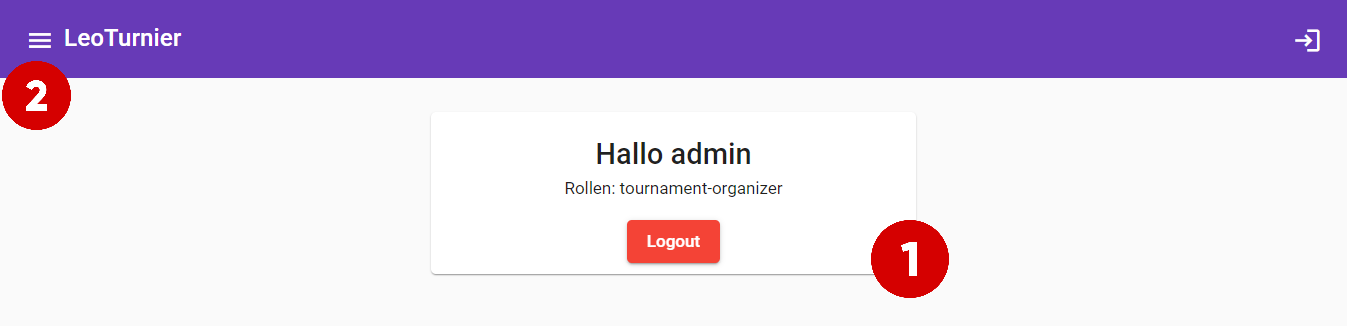
\includegraphics[scale=0.4]{pics/user-guide/login-page.PNG}
\bigskip


\includegraphics[scale=0.05]{pics/user-guide/numbers/number-1.png} \begin{LARGE} Rollen und Logout Button \end{LARGE}

Hier finden Sie alle Ihnen zugewiesenen Rollen sowie einen Logout-Button der ihre Session beendet und Sie zurück zur Home-Page leitet.
\bigskip

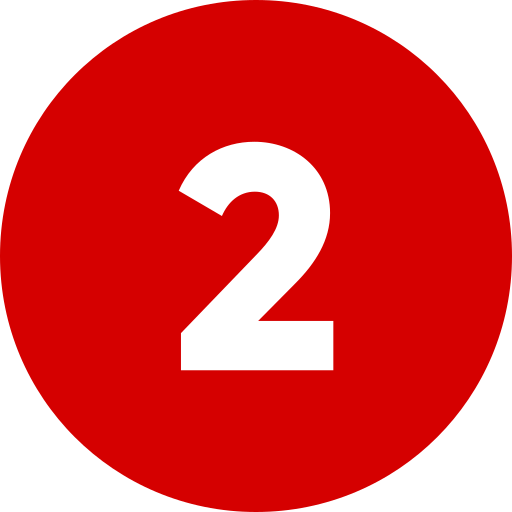
\includegraphics[scale=0.05]{pics/user-guide/numbers/number-2.png} \begin{LARGE} Navigation-Burger \end{LARGE}

Nachdem Sie jetzt eingeloggt sind erscheint oben rechts ein Nav-Burger. Per Knopfdruck zeigt dieser Ihnen nun eine Liste aller Pages die zur
Turnierverwaltung nötig sind.
\section{Player-Page}
\section{Team-Page}
\section{Tournament-Page}
\section{Match-Overview-Page} 